% Template cho một chương

\chapter{Tổng Quan} % Tên của chương

\label{Chapter2} % Thay X bằng số chương tương ứng; để trích dẫn chương này ở chỗ nào đó trong bài, hãy sử dụng lệnh \ref{ChapterX} 

%----------------------------------------------------------------------------------------
%	MỤC 1
%----------------------------------------------------------------------------------------
\newcommand{\keyword}[1]{\textbf{#1}}
\newcommand{\tabhead}[1]{\textbf{#1}}
\newcommand{\code}[1]{\texttt{#1}}
\newcommand{\file}[1]{\texttt{\bfseries#1}}
\newcommand{\option}[1]{\texttt{\itshape#1}}

\section{TensorFlow}
\subsection{TensorFlow là gì?}
Với sự bùng nổ của lĩnh vực Trí Tuệ Nhân Tạo – A.I. trong thập kỷ vừa qua, machine learning và deep learning rõ ràng cũng phát triển theo cùng. 
Và ở thời điểm hiện tại, TensorFlow chính là thư viện mã nguồn mở cho machine learning nổi tiếng nhất thế giới, được phát triển bởi các nhà nghiên 
cứu từ Google. Việc hỗ trợ mạnh mẽ các phép toán học để tính toán trong machine learning và deep learning đã giúp việc tiếp cận các bài toán trở 
nên đơn giản, nhanh chóng và tiện lợi hơn nhiều. 

Hiện nay, TensorFlow cơ bản được xem như một trong những phương tiện trung gian giúp tính toán cho các số lượng có trong sản xuất và đồng thời trở 
thành một công cụ không thể thiếu trong Machine Learning, cùng với sự tương thích với nhiều ngôn ngữ lập trình như C++, Python, Java... 
Từ đó, phục vụ cho nhu cầu học tập cũng như nghiên cứu một cách dễ dàng hơn. 

Tensor được hiểu là một loại cấu trúc dữ liệu được tập hợp 
trong một thư viện mà ở đó chính là TensorFlow. Trong số đó, cấu trúc của dữ liệu sẽ được miêu tả rồi điều chỉnh theo nhiều cách sao cho phù hợp 
nhất với các kiểu dữ liệu này. Và, cấu trúc dữ liệu này sẽ bao gồm 3 thuộc tính chính là: Bậc, chiều và loại dữ liệu. 


Các hàm được dựng sẵn trong thư viện cho từng bài toán cho phép TensorFlow xây dựng được nhiều neural network. 
Nó còn cho phép tính toán song song trên nhiều máy tính khác nhau, thậm chí trên nhiều CPU, GPU trong cùng 1 máy hay tạo ra các dataflow graph – đồ 
thị luồng dữ liệu để dựng nên các model.






\subsection{Cách TensorFlow hoạt động}
Kiến trúc của Tensorflow cơ bản bao gồm 3 phần chính là: 
\begin{itemize}
\item \textbf{Tiền xử lý dữ liệu}
\item \textbf{Dựng Model}
\item  \textbf{Train và ước tính Model}
\end{itemize}

Khi TensorFlow hoạt động sẽ cho phép các lập trình viên có thể tạo ra dataflow graph, cũng như cấu trúc mô tả làm sao để cho dữ liệu có thể di chuyển 
qua 1 biểu đồ; hoặc di chuyển qua 1 seri mà các node đang xử lý. Mỗi một node có trong đồ thị thường đại diện cho 1 operation toán hoặc và mỗi kết nối 
thường hay edge giữa các node với nhau.

Từ đó, mỗi kết nối hoặc edge giữa các node được xem là mảng dữ liệu đa chiều. TensorFlow sẽ cung cấp tất cả mọi điều đến cho lập trình viên dựa theo 
phương thức của ngôn ngữ Python. Ngôn ngữ này sẽ cung cấp nhiều cách tiện lợi để ta có thể hiểu được nên làm thế nào cho các high-level abstractions 
có thể kết hợp được với nhau. Node cũng như tensor có trong TensorFlow chính là đối tượng của Python. Và, mọi ứng dụng Tensorflow bản thân chúng chính 
là một ứng dụng Python. 

Các operation toán học thực sự thì thường không được thi hành bằng Python. Những thư viện biến đổi thường không có sẵn thông qua TensorFlow được viết 
bằng các binary C++ có hiệu suất cao.
Ngoài ra, Python chỉ điều hướng cho các lưu lượng giữa các phần cũng như cung cấp các high-level abstraction lập trình để có thể nối chúng lại với nhau. 
Train thường phân tán dễ chạy hơn nhờ vào API mới và sự hỗ trợ cho TensorFlow Lite để cho phép việc triển khai các mô hình trên với nhiều nền tảng khác nhau. 

\subsection{Adam Optimizer}
Adam là viết tắt của Adaptive Moment Estimation là một thuật toán cho kỹ thuật tối ưu hóa để giảm dần độ dốc. Adam có hiệu quả cao và được sử dụng rộng rãi 
trong các bài toán học máy. Phương pháp này thực sự hiệu quả khi làm việc với bài toán lớn liên quan đến nhiều dữ liệu hoặc tham số. Nó đòi hỏi ít bộ nhớ hơn và hiệu quả. 
Nó là sự kết hợp của thuật toán "gradient descent" và "RMSProp".

\subsubsection*{Gradient descent with momentum}
Thuật toán gradient descent with momentum được sử dụng để tăng tốc thuật toán giảm độ dốc bằng cách xem xét "trung bình trọng số theo cấp số nhân" của độ dốc. 
Sử dụng mức trung bình làm cho thuật toán hội tụ về phía cực tiểu với tốc độ nhanh hơn.

\begin{equation}
\begin{aligned}
m_t & = \beta_1 m_{t-1} + (1 - \beta_1) \frac{\delta L}{\delta w_t} \\
w_t & = w_{t-1} - \alpha m_t\\
\end{aligned}
\end{equation}

trong đó :

\begin{itemize}
\item $m_t$ là tổng các gradient tại thời điểm t. (với $m_0 = 0$)
\item $v_t$ là tổng các gradient tại thời điểm t-1.
\item $\beta$ là tham số trung bình.
\item $\alpha$ là tốc độ học.
\item $\delta L$ là đạo hàm của hàm mất mát.
\item $w_t$ là trọng số tại thời điểm t.
\item $w_{t-1}$ là trọng số tại thời điểm t-1.  
\end{itemize}

\subsubsection*{Root Mean Square Propagation (RMSP)}
Root mean square prop hay RMSprop là một thuật toán học thích ứng cố gắng cải thiện AdaGrad. Thay vì lấy tổng tích lũy của bình phương độ dốc như trong AdaGrad, 
nó lấy "trung bình động hàm mũ".

\begin{equation}
\begin{aligned}
v_t & = \beta v_{t-1} + (1 - \beta) (\frac{\delta L}{\delta w_t})^2 \\
w_t & = w_{t-1} - \alpha_t \frac{\delta L}{\delta w_t} \frac{1}{\sqrt{v_t + \epsilon}}\\
\end{aligned}
\end{equation}

trong đó:

\begin{itemize}
\item $v_t$ tổng bình phương của gradient trong quá khứ.
\item $\beta$ là tham số trung bình.
\item $\alpha$ là tốc độ học.
\item $\delta L$ là đạo hàm của hàm mất mát.
\item $w_t$ là trọng số tại thời điểm t.
\item $w_{t-1}$ là trọng số tại thời điểm t-1.
\item $\epsilon$ là một hằng số dương rất nhỏ để tránh chia cho 0.
\item $\delta w_t$ là đạo hàm của trọng số tại thời điểm t .

\end{itemize}

\textbf{Adam Optimizer} kế thừa các điểm mạnh hoặc thuộc tính tích cực của hai phương pháp trên và dựa trên chúng để tạo ra độ dốc giảm dần được tối ưu hóa hơn.

\subsection*{Công thức toán học của Adam Optimizer}
Từ 2 công thức 1.1 và 1.2 ta có :
\begin{equation}
\begin{aligned}
m_t & = \beta_1 m_{t-1} + (1 - \beta_1) \frac{\delta L}{\delta w_t} \\
v_t & = \beta_2 v_{t-1} + (1 - \beta_2) (\frac{\delta L}{\delta w_t})^2 \\
\hat{m_t} & = \frac{m_t}{1 - \beta_1^t} \hat{v_t} \\
w_t & = w_{t-1} - \alpha_t \frac{\hat{m_t}}{\sqrt{\hat{v_t}} + \epsilon}\\
\end{aligned}
\end{equation}

trong đó:

\begin{itemize}
\item $\beta_1$ và $\beta_2$ tốc độ phân rã trung bình của các gradient trong hai phương pháp trên.
\item $\hat{m_t}$ và $\hat{v_t}$ là các tham số trọng số đã hiệu chỉnh sai lệch.
\end {itemize} 
Từ đó ta thu được:
\begin{equation}
    \begin{aligned}  
    w_t & = w_{t-1} - \alpha_t \frac{\hat{m_t}}{\sqrt{\hat{v_t}} + \epsilon}\\
\end{aligned}
\end{equation}

Dựa trên những điểm mạnh của các mô hình trước đó, trình tối ưu hóa Adam mang lại hiệu suất cao hơn nhiều so với mô hình được sử dụng trước đây và vượt trội hơn
chúng một cách đáng kể trong việc tạo ra độ dốc giảm dần được tối ưu hóa. Biểu đồ được hiển thị bên dưới mô tả rõ ràng cách trình tối ưu hóa của Adam vượt trội 
so với phần còn lại của trình tối ưu hóa bằng một biên độ đáng kể về chi phí đào tạo (thấp) và hiệu suất (cao). 

\begin{figure}[h!]
    \centering
    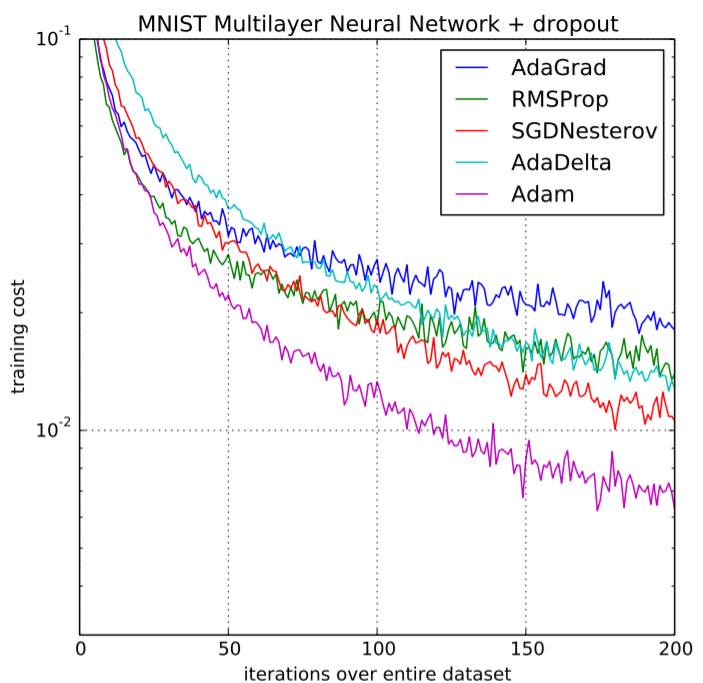
\includegraphics[width=0.8\linewidth]{Image/Adam.png}
    \caption{So sánh các thuật toán tối ưu hóa}
    \label{Hình 1.1: Graph Neural Network}
    \cite*{WEBSITE:3}
\end{figure}


\textbf{Trong TensorFlow} thuật toán tối ưu hóa Adam được sử dụng với các thông số mặc định của các công thức trên là $\alpha$ = 0.001, $\beta_1$ = 0.9, $\beta_2$ = 0.999, và $\epsilon$ = 1e-8. 
Các thông số này có thể dễ dàng tùy biến bằng cách gán các giá trị cho các thuộc tính tương ứng có sẵn trong Adam.


\section{Neural Structured Learning}
Neural Structured Learning (NSL) là một mô hình học tập mới để huấn luyện mạng thần kinh bằng cách tận dụng các tín hiệu có cấu trúc bên cạnh các đầu vào tính 
năng. Cấu trúc có thể rõ ràng như được biểu thị bằng biểu đồ hoặc ẩn khi gây ra "nhiễu loạn đối nghich.

Các tín hiệu có cấu trúc thường được sử dụng để biểu thị các mối quan hệ hoặc sự giống nhau giữa các mẫu có thể được gắn nhãn hoặc không gắn nhãn. Do đó, việc 
tận dụng các tín hiệu này trong quá trình huấn luyện mạng thần kinh sẽ khai thác cả dữ liệu được gắn nhãn và không được gắn nhãn, điều này có thể cải thiện độ 
chính xác của mô hình, đặc biệt khi lượng dữ liệu được gắn nhãn tương đối nhỏ . Ngoài ra, các mô hình được đào tạo với các mẫu được tạo bằng cách thêm nhiễu loạn 
đối nghịch đã được chứng minh là hoạt động tốt đối với các dữ liệu không tốt được thiết kế để đánh lừa dự đoán hoặc phân loại của mô hình.

NSL khái quát hóa thành Neural Graph Learning cũng như Adversarial Learning. Khung NSL trong TensorFlow cung cấp các API và công cụ dễ sử dụng sau đây cho các 
nhà phát triển để đào tạo các mô hình với các tín hiệu có cấu trúc:
\begin{itemize}
    \item \textbf{Keras APIs} để cho phép đào tạo với đồ thị (cấu trúc rõ ràng) và nhiễu đối phương (cấu trúc ngầm định).
    \item \textbf{TF ops and functions} cho phép đào tạo với cấu trúc khi sử dụng các API TensorFlow cấp thấp hơn.
    \item \textbf{Tools} để xây dựng đồ thị và xây dựng đầu vào đồ thị để đào tạo.
\end{itemize}

\begin{figure}[h!]
    \centering
    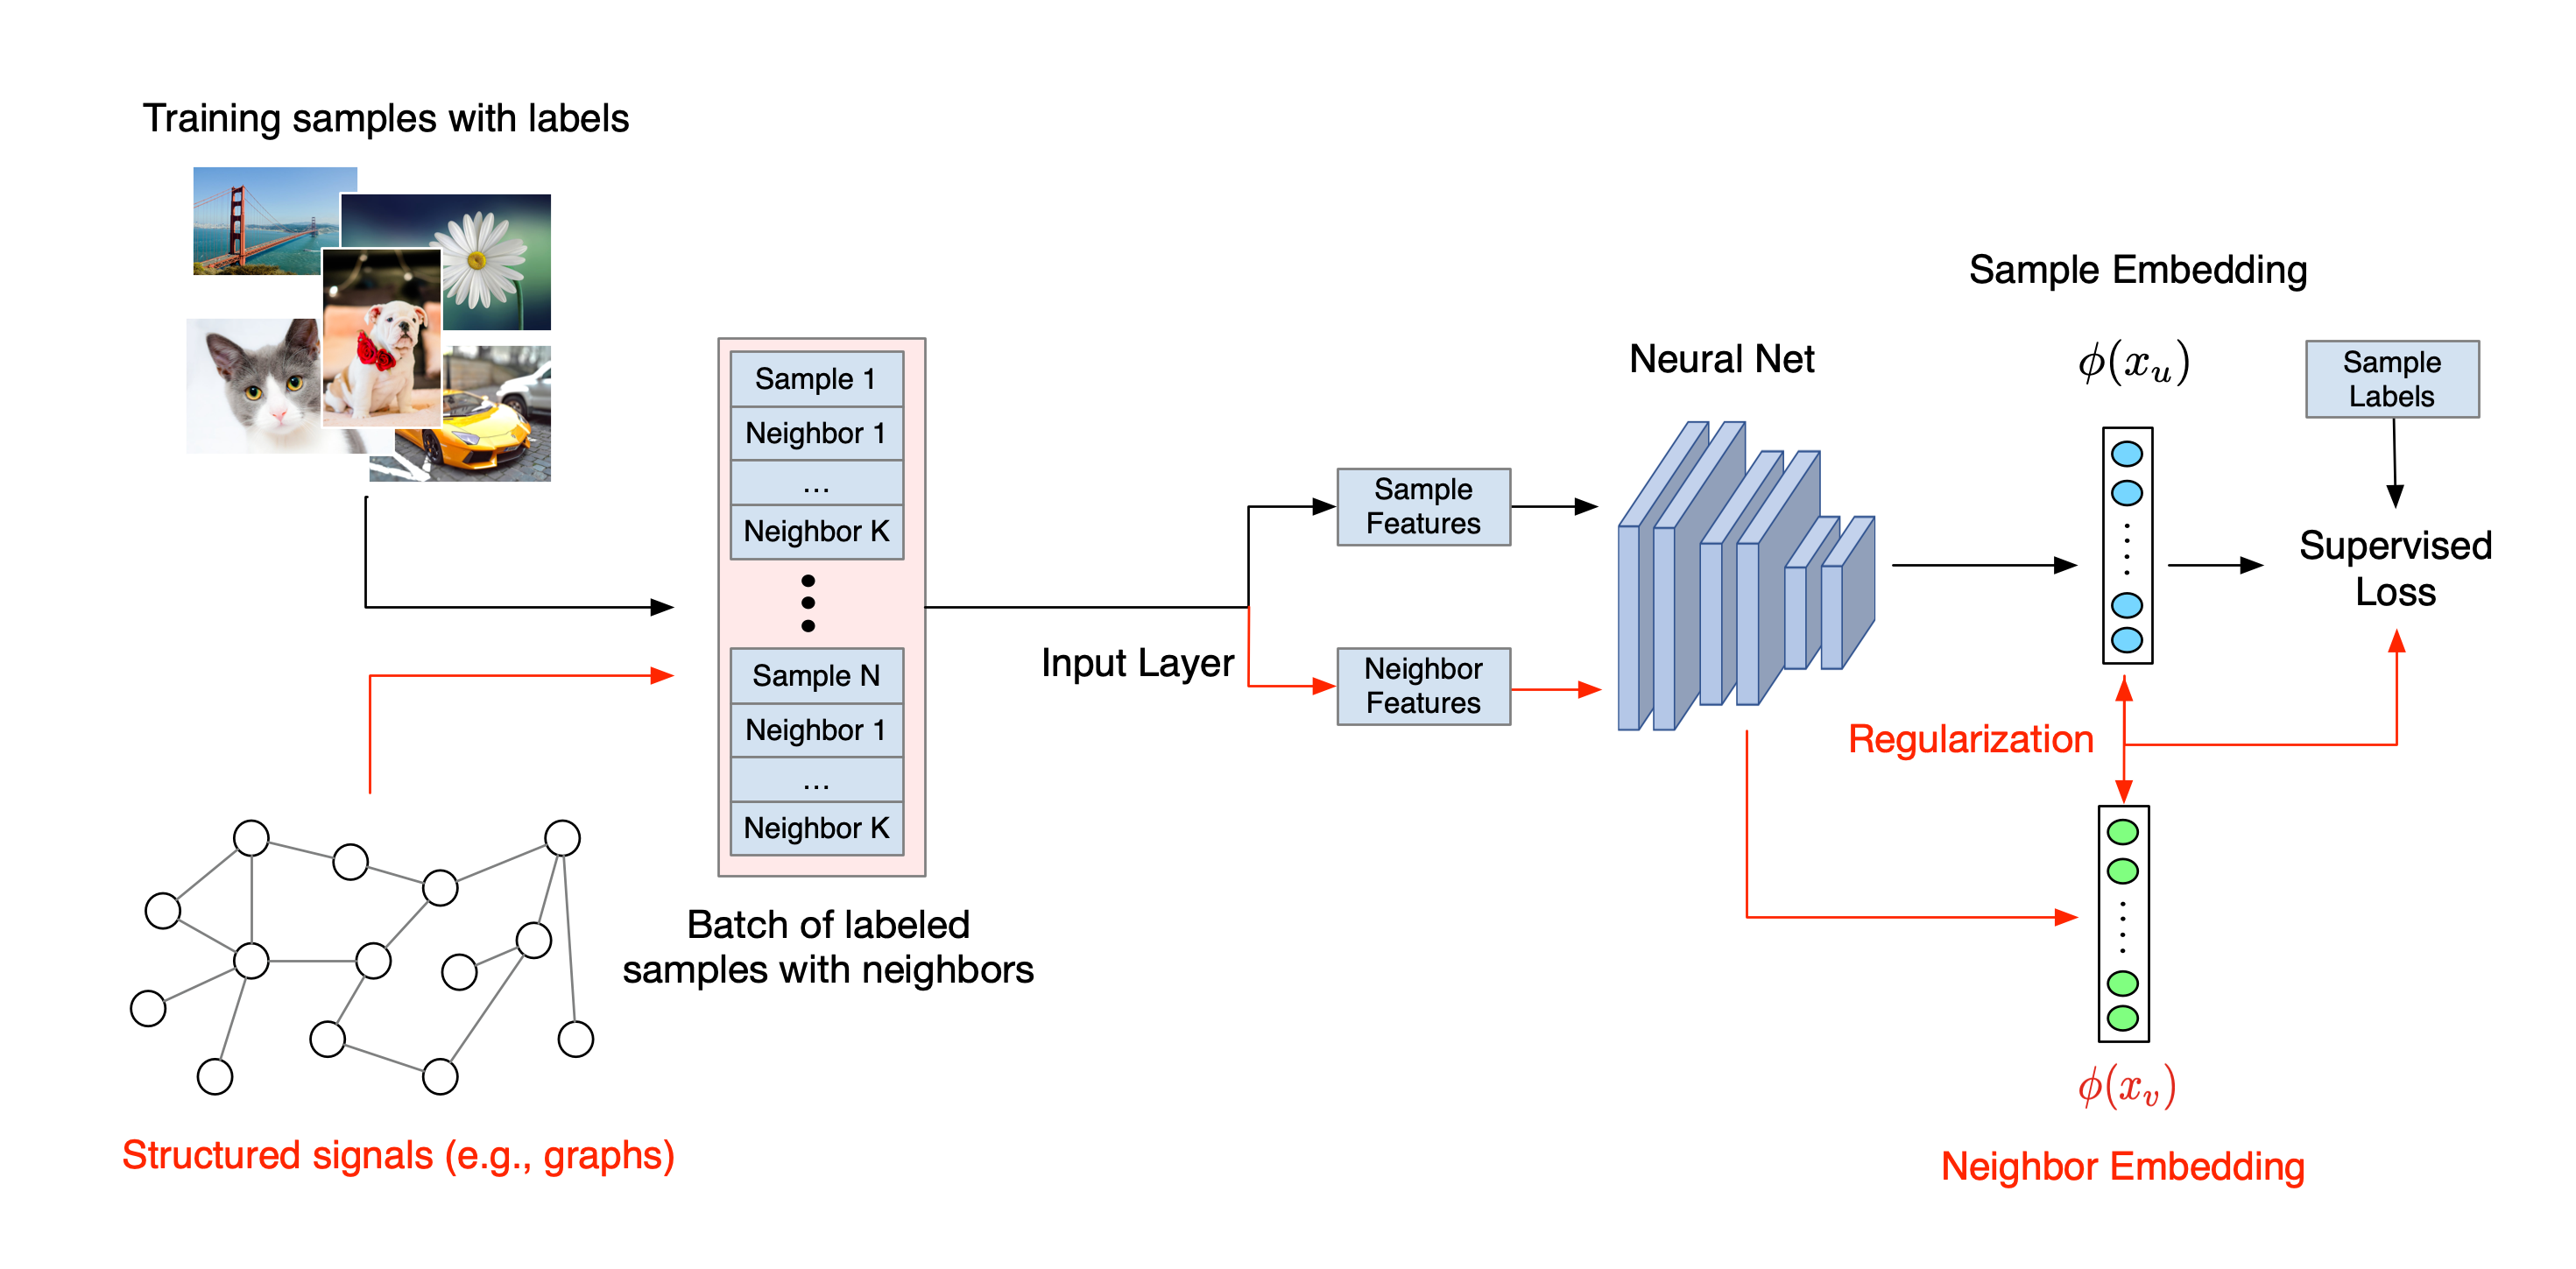
\includegraphics[width=0.8\linewidth]{Image/NSL.png}
    \caption {Neural Structured Learning}
    \label{Hình 1.2: Neural Structured Learning}
    \cite*{WEBSITE:4}
\end{figure}

Trong Neural Structured Learning (NSL), các tín hiệu có cấu trúc dù được xác định rõ ràng dưới dạng biểu đồ hay được học ngầm dưới dạng cách ví dụ đối nghịch được 
được sử dụng để thường xuyên đào tạo mạng neural, buộc mô hình phải học các dự đoán chính xác (bằng cách giảm thiểu mất mát có giám sát), đồng thời duy trì sự giống nhau giữa các đầu vào từ 
cùng một cấu trúc(bằng cách giảm thiểu tổn thất lân cận). Kỹ thuật này là chung và có thể được áp dụng trên các kiến trúc neural tùy ý, chẳng hạn như Feed-Forward NNs, CNNs, RNNs. 


\subsection{Neural Graph Learning}

\textbf{Training with natural graphs}

\begin{figure}[h!]
    \centering
    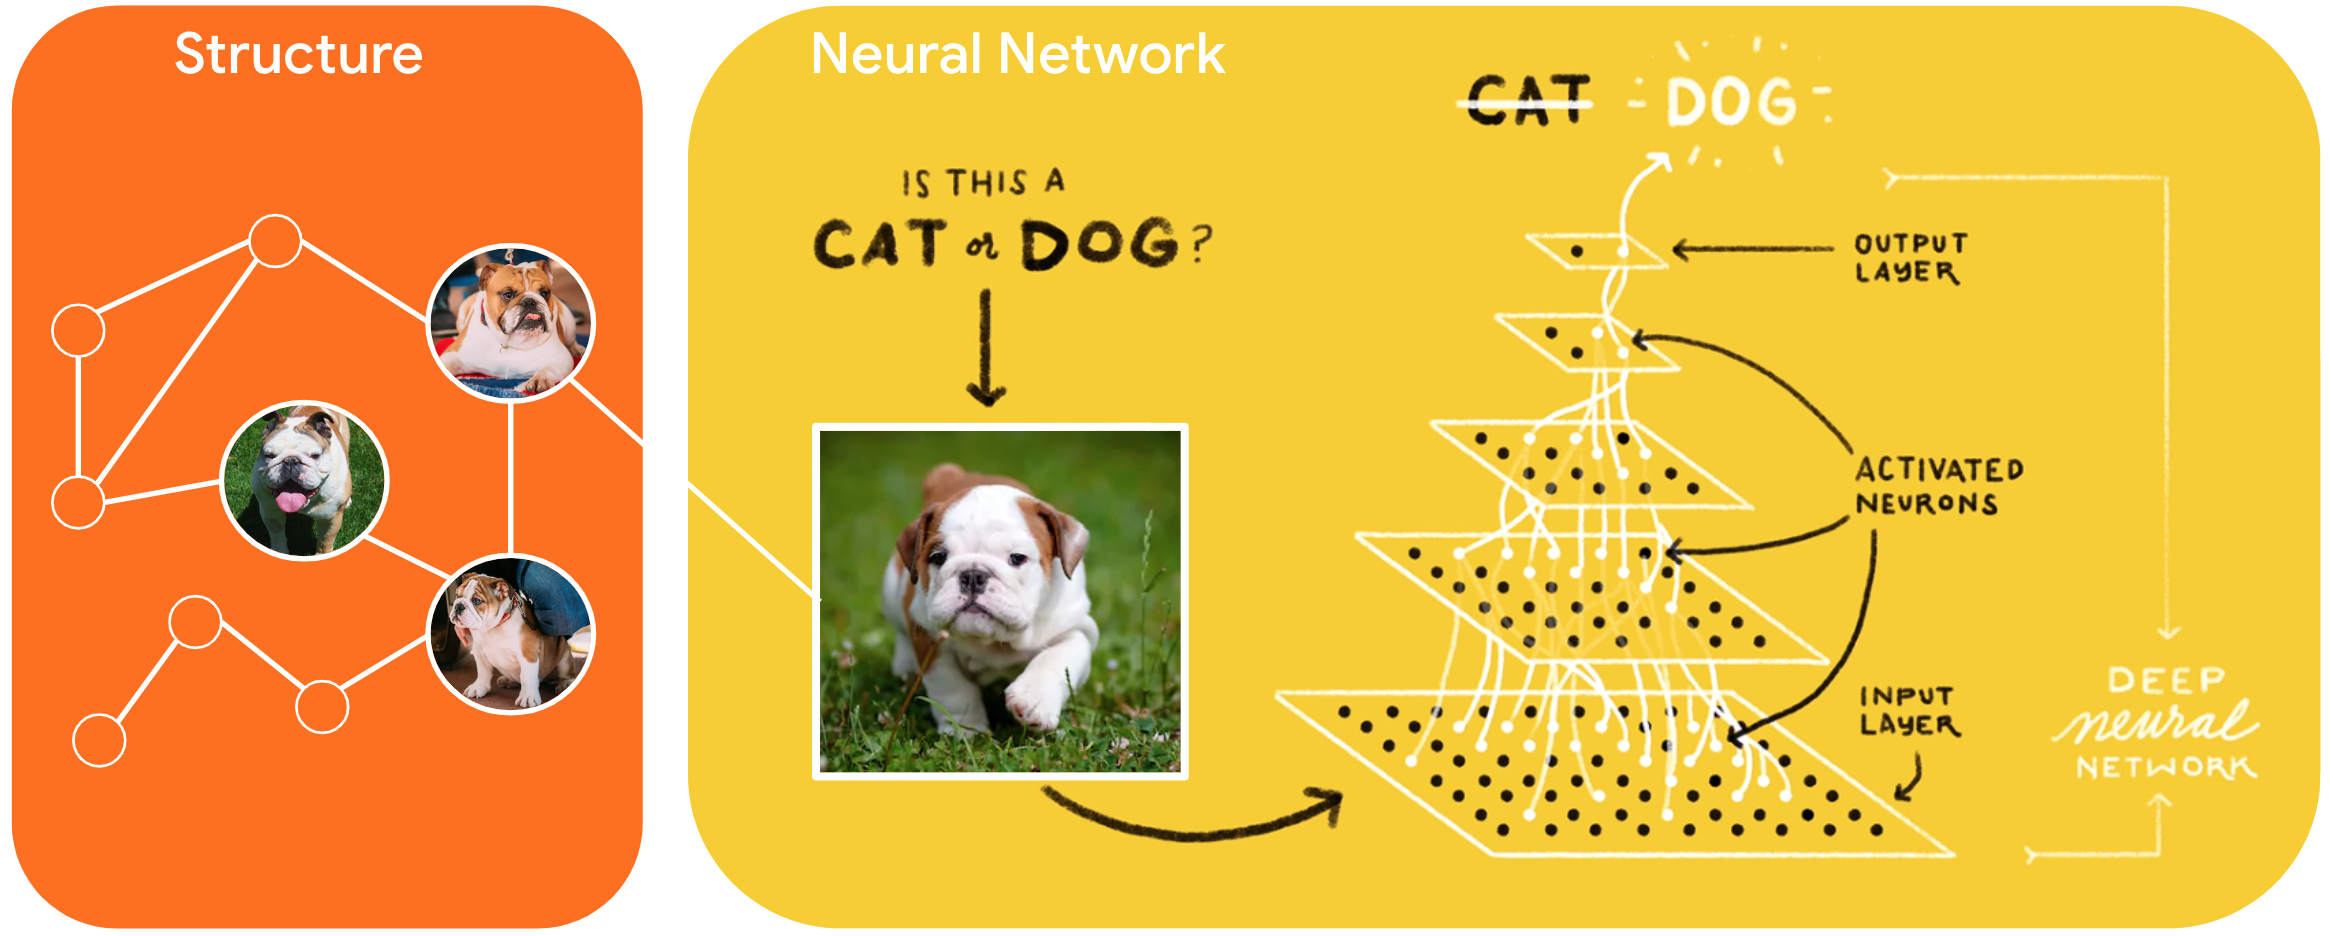
\includegraphics[width=0.8\linewidth]{Image/nsl_overview.png}
    \caption{Training with natural graphs}
    \label{Hình 1.3: Training with natural graphs}
    \cite*{WEBSITE:4}
\end{figure}

Về cơ bản, đồ thị tự nhiên là một tập hợp các điểm dữ liệu có mối quan hệ mật thiết với nhau, bản chất của mối quan hệ này có thể thay đổi dựa trên bối cảnh.
Mạng xã hội và Web là những ví dụ kinh điển mà chúng ta tương tác hàng ngày, ngoài những ví dụ này, chúng còn thường xuất hiện trong dữ liệu thường được sử dụng
cho nhiều nhiệm vụ học máy. Ví dụ khi ta cố gắng nắm bắt hành vi của người dùng dựa trên tương tác của họ với dữ liệu, thì việc lập mô hình dữ liệu dưới dạng biểu đồ 
có thể hợp lý. Đối với xử lý ngôn ngữ tự nhiên, chúng ta có thể định nghĩa một biểu đồ văn bản trong đó các nút biểu thị các thực thể và các cạnh biểu thị mối quan hệ 
giữa các cặp thực thể.

Xem xét bài toán phân loại tài liệu. Ví dụ như những kỹ sư AI thường chỉ quan tâm đến các bài viết về học máy trên một chủ đề cụ thể như thị giác máy tính hoặc xử lý ngôn ngữ
tự nhiên hoặc học tăng cường. Và thông thường, chúng ta có rất nhiều tài liệu hoặc giấy tờ như thế để phân loại, nhưng rất ít trong số chúng có nhãn. Vì vậy cần phải làm cho 
dữ liệu được thiết lập thành một biểu đồ tự nhiên, điều này nghĩa là nếu một bài báo hoặc tài liệu được trích dẫn từ bài báo hoặc tài liệu khác thì chúng có thể có cùng nhãn.
Việc sử dụng các thông tin quan hệ như vậy từ biểu đồ trích dẫn tận dụng được cả các mẫu được gắn nhãn cũng như không được gẵn nhãn. Điều này có thể bù đắp cho việc thiếu nhãn 
trong dữ liệu đào tạo. Vì vậy, việc xây dựng các đồ thị tự nhiên là rất cần thiết để giúp đào tạo các mô hình học máy một cách hiệu quả hơn.

\textbf{Traning with synthesized graphs}

\begin{figure}[h!]
    \centering
    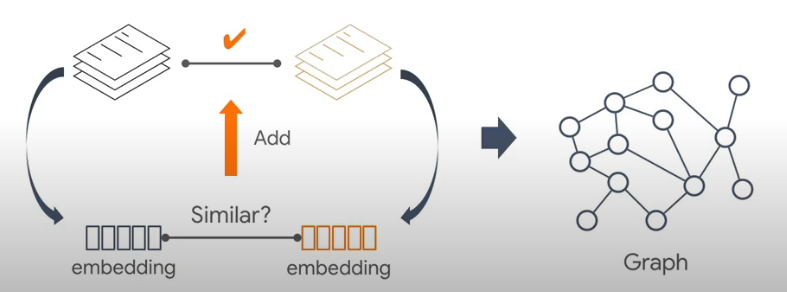
\includegraphics[width=0.8\linewidth]{Image/Graph2.png}
    \caption{Traning with synthesized graphs}
    \label{Hình 1.3: Traning with synthesized graphs}
    \cite*{WEBSITE:4}
\end{figure}

Mặc dù đồ thị tự nhiên là phổ biến, tuy nhiên có nhiều bài toán học máy với dữ liệu đầu vào không tạo thành đồ thị tự nhiên.
Ví dụ như phân loại văn bản đơn giản hoặc phân loại hình ảnh thì dữ liệu đầu vào chỉ chứa hình ảnh hoặc văn bản thô, do đó ta không thể 
tạo ra biểu đồ tự nhiên. Vì vậy Training with synthesized graphs được sử dụng để giải quyết vấn đề này. Với ý tưởng chính là xây dựng hoặc tổng hợp một biểu đồ từ dữ liệu đầu vào.
Trong Training with synthesized graphs chúng ta vẫn sự dụng sự giống nhau giữa các dữ liệu để xây dựng biểu đồ. Để xác định số liệu tương tự, thì cần phải chuyển đổi các văn bản thô hoặc
hình ảnh thành các thành phần nhúng tương ứng hoặc các biểu diễn dày đặc. Khi chuyển đổi dữ liệu thành các thành phần nhúng tương ứng, thì ta có thể sử dụng các mô hình đào tạo trước đó hoặc 
một số hàm chẳng hạn như cos để so sánh mức độ tương ứng giữa của các cặp phần nhúng. Nếu điểm tương đồng lớn hơn một ngưỡng nhất định thì ta sẽ thêm vào một cạnh tương ứng vào biểu đồ kết quả.
Việc lặp lại quy trình này sẽ bao phủ toàn bộ tập dữ liệu và sẽ tạo ra một biểu đồ. Và khi ta có biểu đồ thì việc sử dụng phương pháp học có cấu trúc trung tính rất đơn giản.


\subsection{Adversarial Learning}

\subsubsection*{Adversarial examples}

Adversarial example là các mẫu được tạo ra với những thao tác tinh vi bằng cách thêm vào các nhiễu đối nghịch nhỏ mà mắt người không thể nào nhìn thấy được đã biến nó thành một hình ảnh hoàn toàn khác dưới con mắt kỹ thuật số của thuật 
toán machine learning.

Một số mô hình học máy bao gồm các mạng lưới thần kinh hiện đại nhất, dễ bị sai lệch trước những Adversarial examples. Những mô hình này cho ra kết quả sai các ví dụ chỉ khác một chút so với các ví dụ được phân loại chính xác từ trong tập 
dữ liệu. Ví dụ như khi chúng ta đưa ra đặc điểm của một con gấu trúc thì chúng ta sẽ tìm những đặc trưng của nó như mắt đen, đầu tròn, thân trắng... Nhưng đối với một mạng neural nhân tạo, miễn là khi dữ liệu được đưa vào chạy qua các layer 
đưa ra kết quả trả lời đúng thì nó sẽ tin hình ảnh của dữ liệu đó là con gấu trúc.

\begin{figure}[h!]
    \centering
    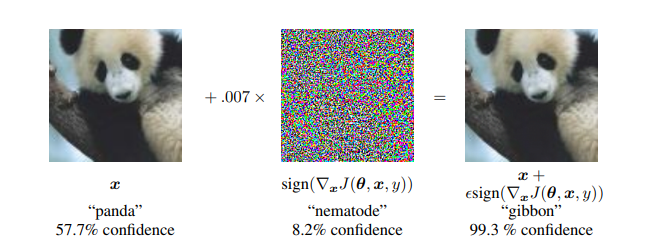
\includegraphics[width=0.8\linewidth]{Image/ADV.png}
    \caption{Adversarial examples}
    \label{Hình 1.4: Adversarial examples}
    \cite*{Reference7}
\end{figure}

Từ hình 1.4 ta thấy, khi thêm vào 1 vector tín hiệu nhiễu rất rất bé mà mắt người không thể phân biệt được sự khác nhau giữa hai hình ảnh của con gấu trúc thì nó đã đánh lừa được mạng neural và khiến nó phán đoán sai và nó tin chắc rằng
thứ mà nó đang nhìn thấy là con vượn (99.3\%). Điều này cho thấy khi các tập dữ liệu không tốt(có nhiễu) thì có thể khiến mạng neural đưa ra phán đoán sai.
 Để giải quyết vấn đề này, Adversarial training được đề xuất để dạy các mạng neural không bị đánh lừa và phân loại sai. 

\cite*{Reference6}
\textbf{Adversarial training}

Khái niệm về Adversarial training liên quan đến việc đào tạo bộ phân loại để khái quát hóa
Adversarial examples cũng như mẫu sạch. Trong lược đồ đào tạo thông thường, được hiển thị trong Hình 1.5, dữ liệu đào tạo chuyển tiếp
thông qua mô hình và tổn thất dự đoán được lan truyền ngược để cải thiện phân loại
kết quả. Kết quả là, mô hình sẽ khái quát hóa việc phân phối dữ liệu huấn luyện để
đưa ra một dự đoán chính xác về nhãn. 

Để đào tạo mô hình tránh bị nhầm lẫn khi tập dữ liệu có nhiễu thì ta sẽ tạo ra các dữ liệu có nhiễu nhỏ từ tập dữ liệu đào tạo
sau đó thêm các cạnh để kết nối dữ liệu vừa tạo ra với các mẫu của nó để xây dựng một cấu trúc linh hoạt sau đó, cấu trúc này có thể được sử dụng trong khung học tập
của cấu trúc thần kinh. Trong khung học cấu trúc thần kinh, mạng thần kinh cố gắng học cách duy trì cấu trúc bằng cách giữ sự giống nhau giữa một mẫu và hàng xóm của nó.
 Vì vậy về cơ bản việc sử dụng tập dữ liệu sạch và dữ liệu đối nghịch của nó sẽ nói với mạng thần kinh rằng mẫu và mẫu đối nghịch của nó thực sự giống nhau. Vì vậy, hãy giữ sự 
 giống nhau giữa chúng và đừng bị nhầm lẫn bởi các nhiễu.

\begin{figure}[h!]
    \centering
    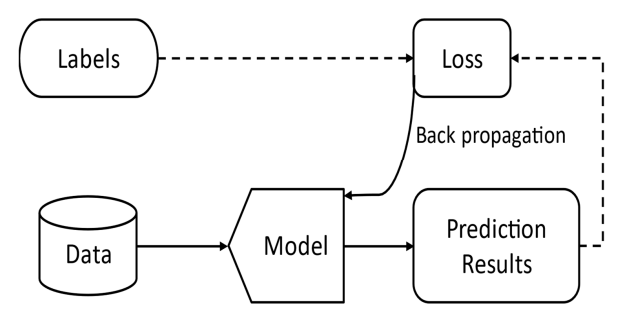
\includegraphics[width=0.72\linewidth]{Image/ADVT1.png}
    \caption{Basic training}
    \label{Hình 1.5: Adversarial training}
    \cite*{Reference8}
\end{figure}

Adversarial training mở rộng các phương pháp đào tạo thông thường bằng cách bổ sung thêm
bước vào quy trình đào tạo, như được minh họa trong Hình 1.6. Bằng cách này, mô hình có thể
khái quát hóa cả dữ liệu sạch và dữ liệu đối nghịch được tạo ra bởi các phương thức
được sử dụng trong Adversarial training để chống lại sự đánh lừa của mẫu đối nghịch.

\begin{figure}[h!]
    \centering
    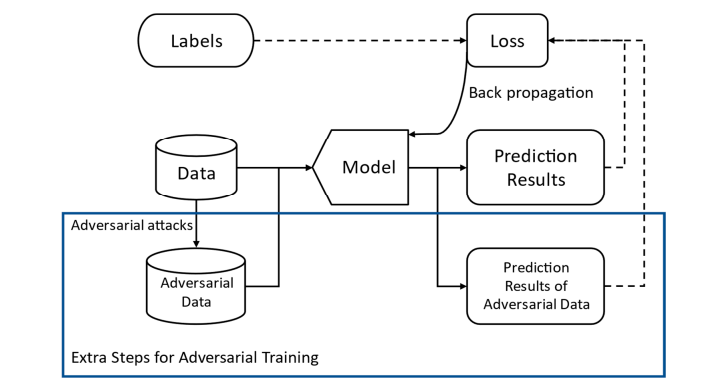
\includegraphics[width=0.72\linewidth]{Image/ADVT2.png}
    \caption{Adversarial training}
    \label{Hình 1.6: Adversarial training}
    \cite*{Reference8}
\end{figure}

Trong thư viện TensorFlow có sẵn các hàm chức năng để tạo ra các mẫu đối ngịch. 
Tương tự thì Keras API cũng có thể sử dụng để cho phép đào tạo từ đầu đến cuối
một cách dễ dàng với Adversarial training như: AdversarialRegularization, AdvNeighborConfig, AdvRegConfig...